% -----------------------------------------------
% Template for SMAC SMC 2013
% adapted and corrected from the template for SMC 2012, which was adapted from that of SMC 2011
% further updated for TENOR 2015, 2016, 2017 and 2018
% -----------------------------------------------

\documentclass{article}
\usepackage{tenor}
\usepackage{ifpdf}
\usepackage[english]{babel}
\usepackage{balance}
\usepackage{listings}


%%%%%%%%%%%%%%%%%%%%%%%% Some useful packages %%%%%%%%%%%%%%%%%%%%%%%%%%%%%%%
%%%%%%%%%%%%%%%%%%%%%%%% See related documentation %%%%%%%%%%%%%%%%%%%%%%%%%%
%\usepackage{amsmath} % popular packages from Am. Math. Soc. Please use the 
%\usepackage{amssymb} % related math environments (split, subequation, cases,
%\usepackage{amsfonts}% multline, etc.)
%\usepackage{bm}      % Bold Math package, defines the command \bf{}
%\usepackage{paralist}% extended list environments
%%subfig.sty is the modern replacement for subfigure.sty. However, subfig.sty 
%%requires and automatically loads caption.sty which overrides class handling 
%%of captions. To prevent this problem, preload caption.sty with caption=false 
%\usepackage[caption=false]{caption}
%\usepackage[font=footnotesize]{subfig}


% REDEFINE THESE VARIABLES:
\def\papertitle{Symbolist: bidirectional mapping developements}
\def\firstauthor{Rama Gottfried}
\def\secondauthor{James Tsz-Him Cheung}
\def\thirdauthor{Georg Hajdu}

\def\copyrightyear{2022}


\usepackage{xspace}
\def\symbolist{\textsc{symbolist}\xspace}
\def\drawsocket{\textsc{drawsocket}\xspace}
\makeatletter
\newcommand{\verbatimfont}[1]{\renewcommand{\verbatim@font}{\ttfamily#1}}
\makeatother


%% Depending on the number of authors, set this variable accordingly for the copyright notice:
% \def\copyrightauthors{Author One}
\def\copyrightauthors{Rama Gottfried, James Cheung and Georg Hajdu}
% \def\copyrightauthors{Author One, Author Two et al}

% adds the automatic
% Saves a lot of output space in PDF... after conversion with the distiller
% Delete if you cannot get PS fonts working on your system.

\def\oscfontsize{\footnotesize}


% pdf-tex settings: detect automatically if run by latex or pdflatex
\newif\ifpdf
\ifx\pdfoutput\relax
\else
   \ifcase\pdfoutput
      \pdffalse
   \else
      \pdftrue
\fi

\ifpdf % compiling with pdflatex
  \usepackage[pdftex,
    pdftitle={\papertitle},
    pdfauthor={\firstauthor},
    bookmarksnumbered, % use section numbers with bookmarks
    pdfstartview=XYZ % start with zoom=100% instead of full screen; 
                     % especially useful if working with a big screen :-)
   ]{hyperref}
  %\pdfcompresslevel=9

  \usepackage[pdftex]{graphicx}
  % declare the path(s) where your graphic files are and their extensions so 
  %you won't have to specify these with every instance of \includegraphics
  \graphicspath{{./figures/}}
  \DeclareGraphicsExtensions{.pdf,.jpeg,.png}

  \usepackage[figure,table]{hypcap}

\else % compiling with latex
  \usepackage[dvips,
    bookmarksnumbered, % use section numbers with bookmarks
    pdfstartview=XYZ % start with zoom=100% instead of full screen
  ]{hyperref}  % hyperrefs are active in the pdf file after conversion

  \usepackage[dvips]{epsfig,graphicx}
  % declare the path(s) where your graphic files are and their extensions so 
  %you won't have to specify these with every instance of \includegraphics
  \graphicspath{{./figures/}}
  \DeclareGraphicsExtensions{.eps}

  \usepackage[figure,table]{hypcap}
\fi

%setup the hyperref package - make the links black without a surrounding frame
\hypersetup{
    colorlinks,%
    citecolor=black,%
    filecolor=black,%
    linkcolor=black,%
    urlcolor=black
}


% Title.
% ------
\title{\papertitle}

 \threeauthors
   {\firstauthor} { University for Music and Theater \\ Hamburg, Germany \\
     {\tt \href{mailto:rama.gottfried@hfmt-hamburg.de}{rama.gottfried@hfmt-hamburg.de}}}
   {\secondauthor} {University for Music and Theater \\ Hamburg, Germany  \\ 
     {\tt \href{mailto:tsz.him.cheung@hfmt-hamburg.de}{tsz.him.cheung@hfmt-hamburg.de}}} 
   {\thirdauthor} {University for Music and Theater \\ Hamburg, Germany \\
     {\tt \href{mailto:georg.hajdu@hfmt-hamburg.de}{georg.hajdu@hfmt-hamburg.de}}}


% ***************************************** the document starts here ***************
\begin{document}
%
\capstartfalse
\maketitle
\capstarttrue


% ABSTRACT
% fill in after finishing the paper
\begin{abstract}

maybe already start with history here, and then continue to symbolist?

  \symbolist is an in-development application for experimental notation, with the goal of creating a working environment for developing symbolic notation for multimedia which can be interpreted and performed by electronics. The program aims to provide an open play space, with tools for experimentation, and thinking visually about relationships between representation and interpretation in media performance. 
In the paper we discuss the evaluation and re-design of the application based on the need for a bi-directional mapping framework for working with symbolic notation and its corresponding data representations.

\end{abstract}


% INTRO
% not sure what should go here, or how in detail to go
% I guess:
% why did I make it, what is it, breifly discuss some of the steps

\section{Background}\label{sec:background}


The \symbolist project was developed out of an organic  

of compositional notation practice. 

how much of a background?


In this paper we present a case study for the creation of an open system for graphically developing symbolic notation which can function both as professional quality print or online documentation, as well as a computer performable score in electro-acoustic music and other computer aided contexts. Leveraging Adobe Illustrator’s graphic design tools and support for the Scalable Vector Graphics (SVG) file format~\cite{world2000scalable}, the study shows that SVG, being based on Extensible Markup Language (XML), can be similarly used as a tree-based container for score information. In the study, OpenSoundControl (OSC)~\cite{wright:osc}  serves as middleware used to interpret the SVG representation and finally realize this interpretation in the intended media context (electronic music, spatial audio, sound art, kinetic art, video, etc.). The paper discusses how this interpretive layer is made possible through the separation of visual representation from the act of rendering, and describes details of the current implementation, and outlines future developments for the project.

Initially developed as a method for performing vector graphics, 
SVG-OSC  \cite{gottfried2015svg}

\cite{maccallum2015dynamic} %middleware
\cite{freed2014io} %io


XML nature of SVG makes it easy to parse and map just like and OSC bundle.

drawing on the OSC research at CNMAT, 

just like a piece of paper, SVG could be freely mappable, and \textit{performable} like OSC.





however it can require a lot of specialized code to handle different hierarchy structures and data at different levels in the hierarchy.


the first version of \symbolist was created as a standalone JUCE application
Ircam/ZKM~\cite{gottfried2018symbolist}

% this can probably be in the backstory part
\subsection{JUCE Version}\label{sec:juce_version}

explain juce version (include in overview?)
MVC~\cite{krasner1988description}
focused on creating SVG and outputting OSC version (like SVG-OSC approach)


\subsection{Clefs and Bidirectional Mapping}\label{sec:bidirectional_mapping}

telling story of how we got where we are, conceptual steps

idea of Clefs

problem:
a lot of mapping is still needed

\subsection{Drawsocket}\label{sec:drawsocket}


\section{Symbolist Electron}\label{sec:symbolist_electron}

using \drawsocket as front end handler \cite{gottfried2019drawsocket}

\cite{hajdu2005quintet}

a general overview about need for classes (actually this comes later when we get into the the discussion of format i.e. the way the data is represented.

js and \drawsocket makes that easy(-ier)


Figure~\ref{fig:screenshot} shows a screenshot from the Electron version.


% screenshot
\begin{figure*}[ht!]
\centering
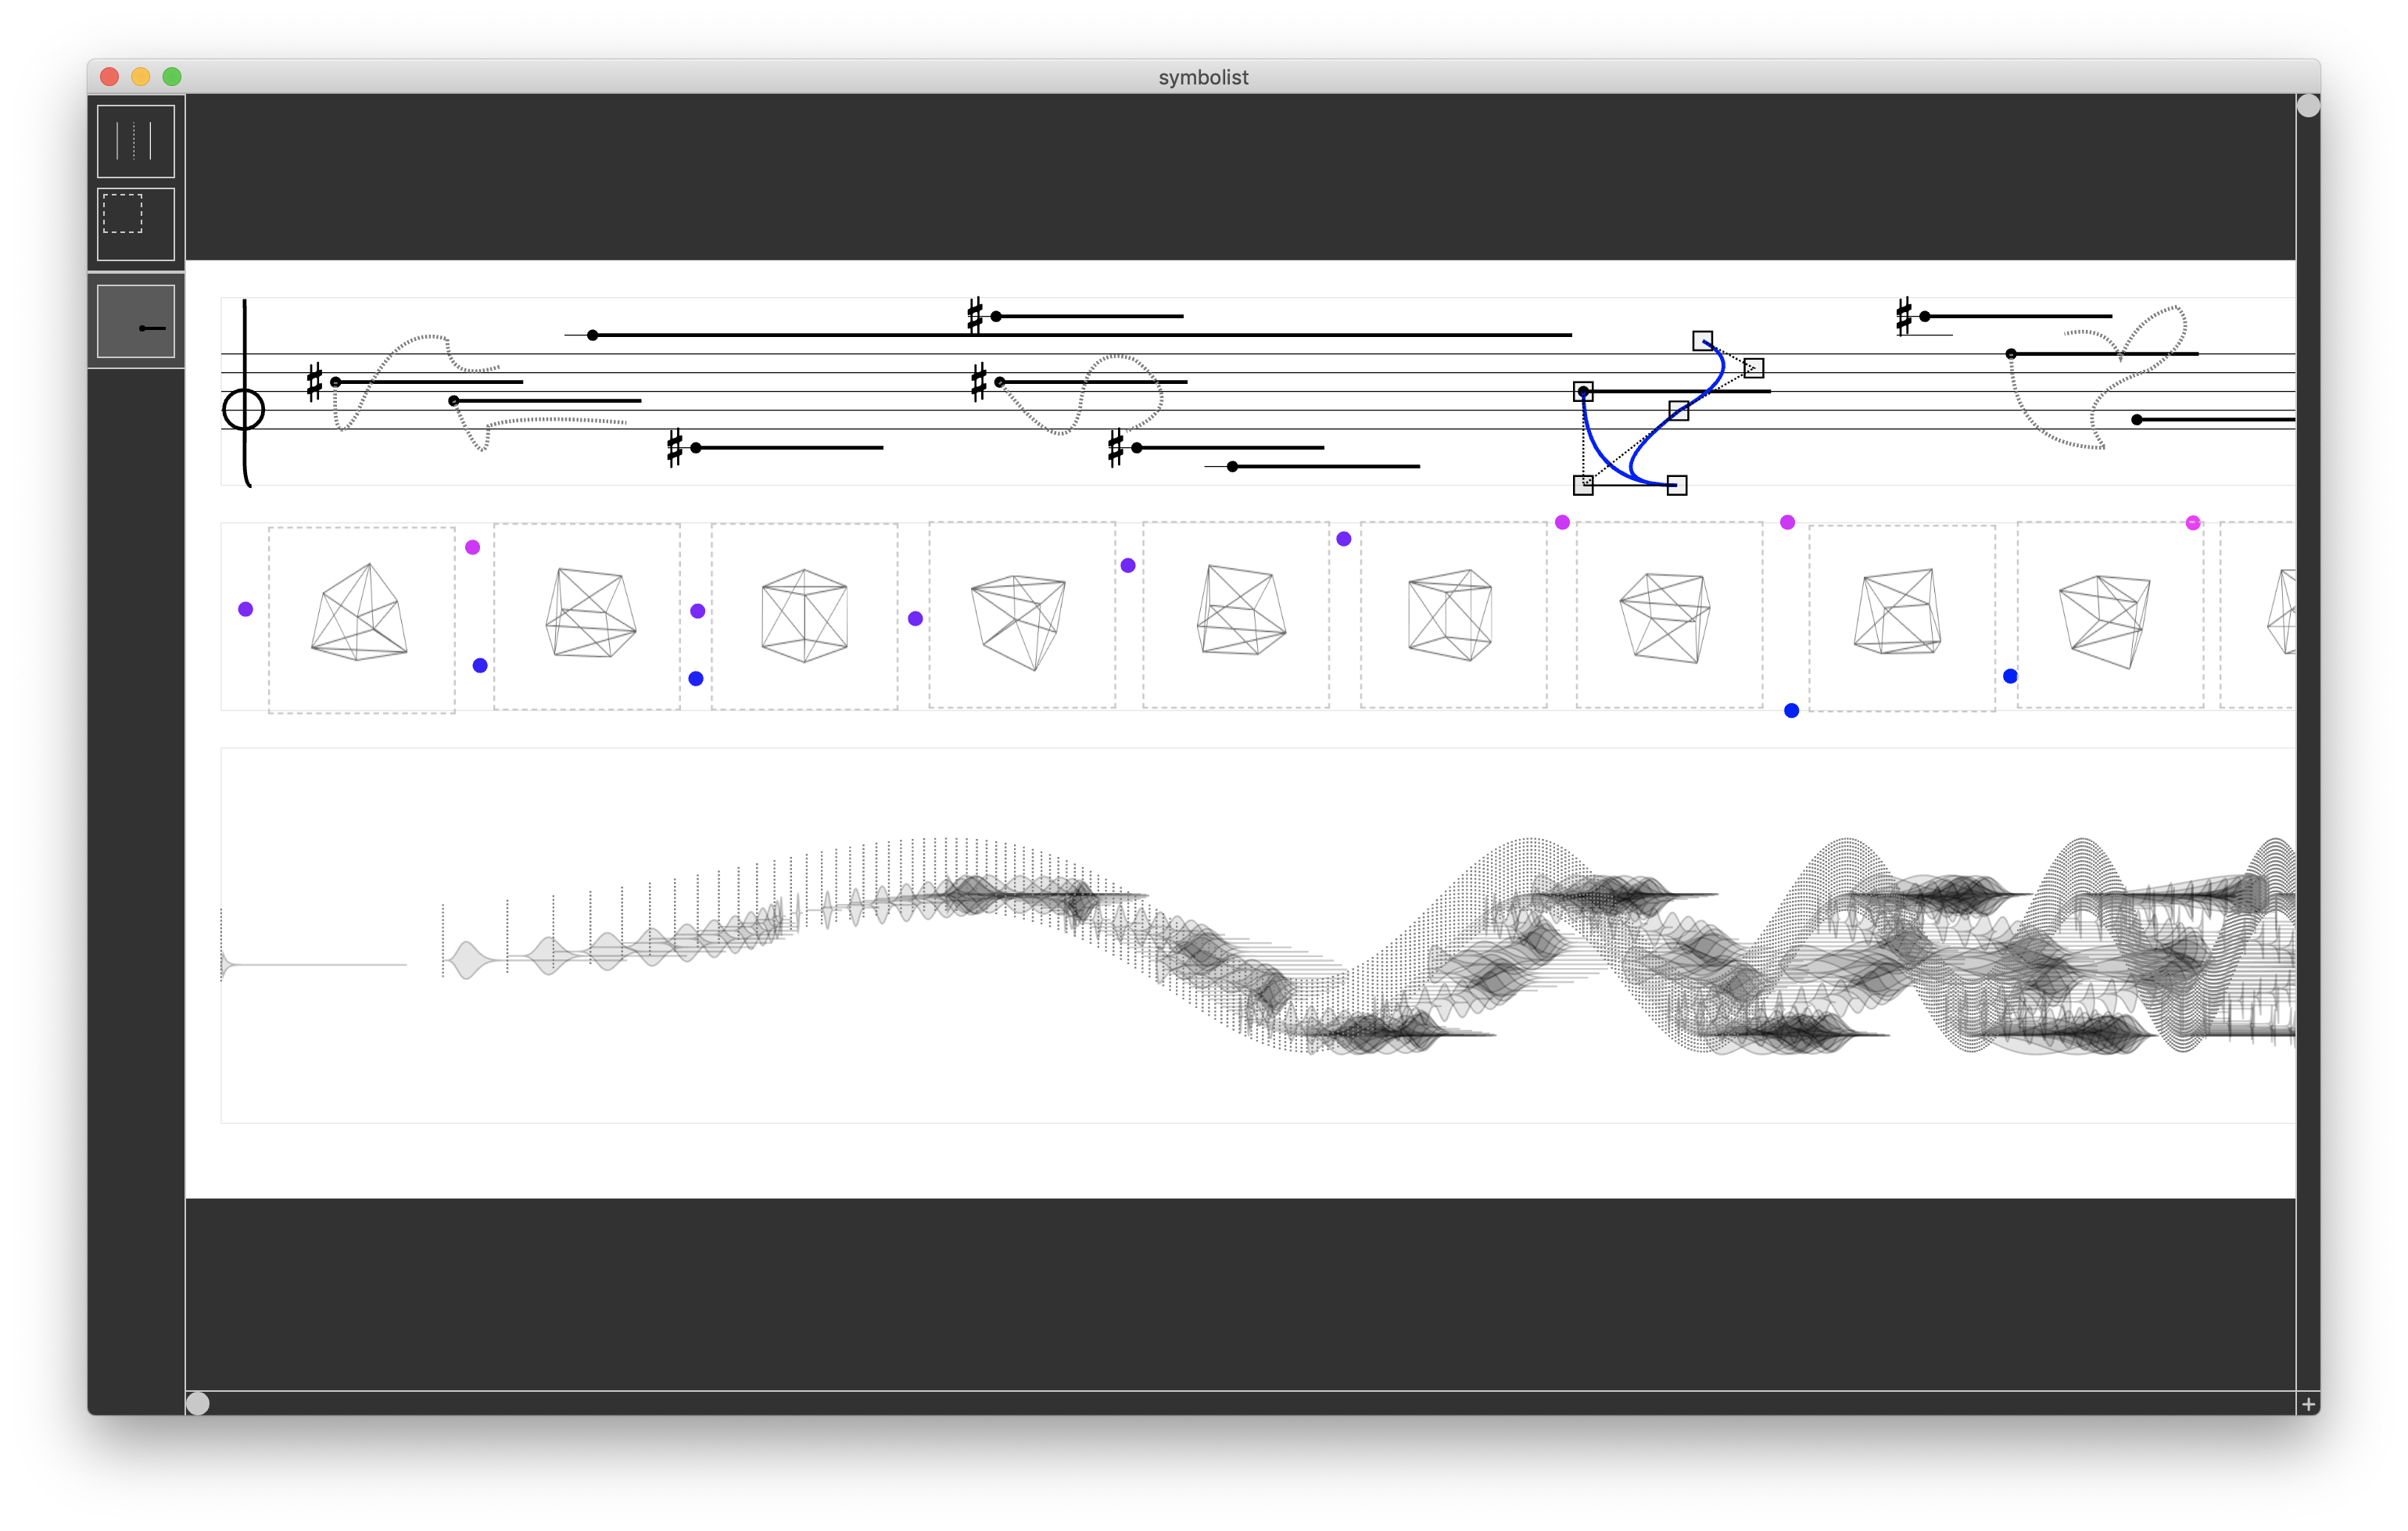
\includegraphics[width=2\columnwidth]{symbolist.png}
\caption{ \symbolist screenshot, showing some different types of staves, and editing capabilities.
\label{fig:screenshot}}
\end{figure*}


\section{Implementations}\label{sec:implementations}

Electron\footnote{https://www.electronjs.org/} version (node + chrome w/ special electron IPC)
Max version (node + jweb + Max patch for IPC)


\begin{figure*}[ht!]
\centering
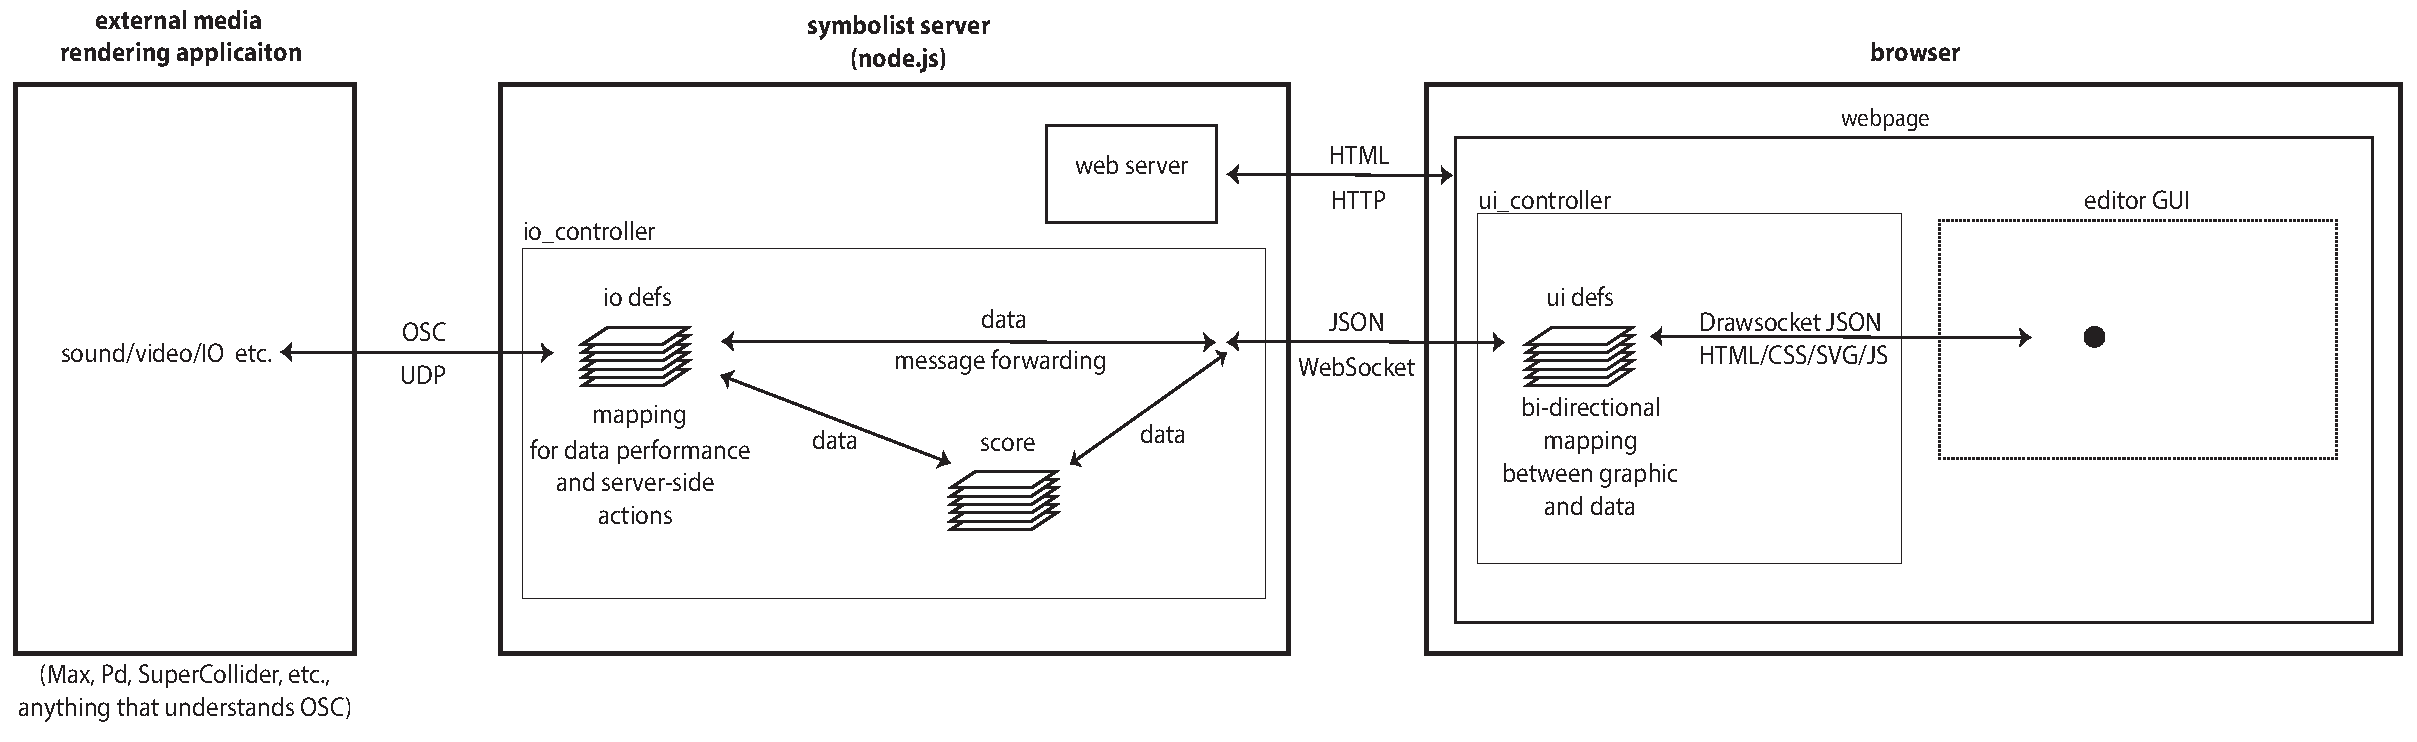
\includegraphics[width=2\columnwidth]{symbolist-architecture2.pdf}
\caption{ \symbolist architecture.
\label{fig:architecture}}
\end{figure*}


\subsection{Application Structure}\label{subsec:application_structure}

The main architecture of the platform (figure~\ref{fig:architecture}) is organized as a server-client model, comprising of:

\begin{enumerate}\itemsep0pt 
\item The \textit{editor}, a browser-based user interface client which displays the graphic representation of the data, and allows the user to edit and create new data objects through graphic interaction. The \textit{ui\_controller} runs in the browser handling interaction, via a library of definition scripts which specify mappings to and from data and graphics formats, as well as other tools and interactions.

\item The \textit{symbolist server}, which is comprised of: 
\begin{itemize}\itemsep0pt 

\item A node.js (Electron) based web-server which serves the main editor webpage via HTTP, and routes messages between the \textit{ui\_controller} and the \textit{io\_controller} via WebSockets, and handles operating system commands like reading and writing files.

\item  The \textit{io\_controller} script runs inside the \textit{symbolist server} and handles input and output from external sources via OSC over a UDP socket. The \textit{io\_controller} holds a copy of the score in its semantic format, and loads a parallel library of user scripts to the \textit{ui\_controller} which define the mapping to (and potentially from) other media sources. The \textit{io\_controller} can also be used to reformat the score into a format that can be performed by another sequencing tool or program like MaxMSP.
\end{itemize}

\end{enumerate}


\section{Graphical Authoring and Interaction}\label{editor} %should this be before or after the application structure?

%the palette symbol system is interesting maybe, to discuss how you can ``enter into'' a symbol, and then the possible sub-elements populate the palette.

The graphic user interface of \symbolist is designed around the idea of symbol objects and containers. Graphic objects, or \textit{symbols} are placed in \textit{container} references which define a framing used to interpret the meaning of the \textit{symbol}.

In order to maintain an open and un-opinionated approach to authoring tools, \symbolist tries not to specify how containers and symbols should look, act, or respond when you interact with them within the application. Rather, the interaction and meanings of the symbols are defined in a library of object \textit{definitions} which create these meanings through mapping semantic data to and from the graphic visualization. Definitions can be shared and loaded to setup different composition environments.

%See below for more information about the API for creating symbol definitions. 

\subsection{Interface Components}\label{subsec:interface_components}

%main interesting thing to talk about is the palette system

The \symbolist graphic editor (shown in figure~\ref{fig:screenshot}) provides a set of basic tools for creating scores using the defined symbols and containers:
\begin{itemize}\itemsep0pt 
\item \textit{document view}: the top level view of the application window.
\item \textit{menu bar}: the menu bar at the top of the screen or window, which provides access to various application functions.
\item \textit{palette}: a set of buttons on in the side bar of the program which display icons of the \textit{symbols} that have been defined for the current selected \textit{container}. 
\item \textit{tools}: a set of buttons that open tools for custom computer-assisted generation of new symbols, and applying transformations to existing elements (e.g. alignment of multiple objects, or setting distributing objects, etc.)
\item \textit{inspector}: a contextual menu for editing the semantic data of an object, which is then mapped to the graphic representation.
\end{itemize}

\subsection{Modes}
maybe this should just be a list
\subsubsection{Palette and Creation}
\subsubsection{Selection, Click and Drag}
\subsubsection{Inspector}
\subsubsection{Edit}


\subsection{User Experience}\label{ux}

On entering the application, the editor loads a score or initialization file from the default load folder, or you can load a new config file after loading. The config file sets the top-level page setup and palette options.

A typical sequence of creating a score might be as follows:
\begin{enumerate}\itemsep0pt
\item The user opens a workspace, with one or more containers displayed on the screen, for example an empty rectangle which is like a piece of paper.
\item Selecting the ``paper'' container rectangle, the user then sets the container as the new \textit{context}, by pressing the [s] key (or selecting from the application menu).
\item Once setting the context, the \textit{palette} toolbar is populated with icons of symbols that are defined with the selected container context type.
\item Clicking on one of the symbol icons, puts the interface into \textit{creation} / \textit{palette mode}, where the mouse interaction is now designed for use with this specific symbol type.
\item Holding the CMD button, creates a preview of the symbol how it will appear when you click, and some text is displayed near the mouse that shows the semantic data associated with the graphic representation.
\item After clicking the symbol is placed in the container.
\item Depending on the symbol type, you may be able to drag the symbol to a new place in the container, and the associated data is updated as a result.
\item Selecting the symbol and hitting the [i] button, brings up the inspector window, where you can edit the data and see the graphics updated in response.
\item Selecting and pressing the [e] button enters \textit{edit mode} which is a modal context where different user interaction could change the values of the symbol in different ways. For example in edit mode you might be able to rotate an object in a certain way, or be able to visualize different connections to the graphic representation to other elements of the score which are not usually highlighted in the score view.
\end{enumerate}




\section{Data Representation}\label{subsec:representation}

At the heart of \symbolist are two parallel forms of information expression: \textit{semantic data} and \textit{graphic representation} (figure~\ref{fig:graphic-representation}).

\textit{Semantic data} specifies the various attributes of information about a symbolic object, in terms of the object's meaning to the author. 
For example, the meaningful attributes of a \textit{note} object might be information about pitch and duration, or a \textit{point} object might contain x, y, and z values corresponding to the point's location in 3D space. In \symbolist \textit{semantic data} is thought of as the main holder of information in the system, which arranged as a score can function like a database of hierarchal information (further explained in section \ref{subsec:file_format} below).

The \textit{graphic representation} of the information is a visual representation of the semantic data, which is open in nature. The aim of \symbolist is to provide an agnostic framework for developing visual, symbolic, or other unknown representations of semantic data for use in multimedia composition practice; and so, one of the main functions of the new version of the software is to facilitate the creation of mapping relationships between different representations of the data (see figure~\ref{fig:graphic-representation}).


\begin{figure}[ht!]
\centering
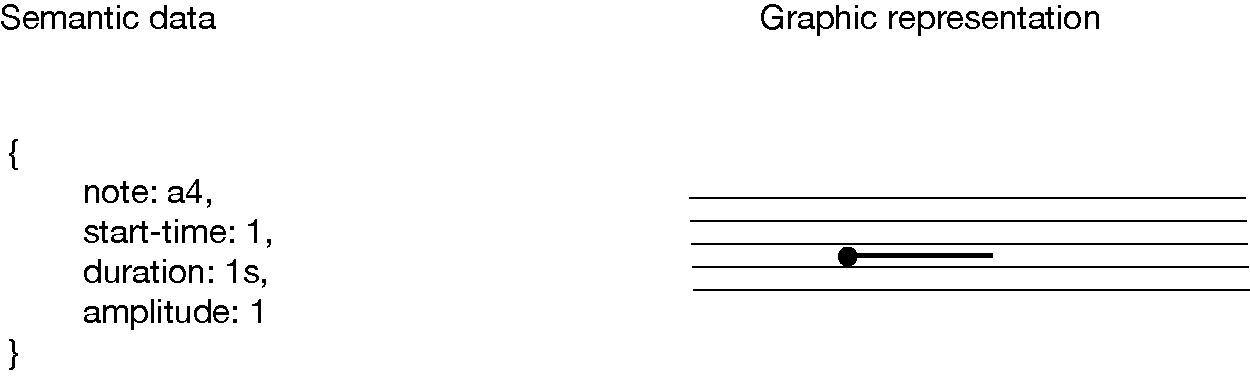
\includegraphics[width=1\columnwidth]{graphic-representation.pdf}
\caption{\textit{data} vs \textit{graphic} representation of the same information.
\label{fig:graphic-representation}}
\end{figure}



\section{Symbols}\label{subsec:symbols}

In \symbolist terminology a \textit{symbol} is an instance of a symbolic representation of data that connects the semantic, graphic, and possibly other media types of expression together as a multifaceted unit.
Each \textit{symbol} is defined as a \textit{class} of object, which specifies the symbol's data structure and UI interaction, and data mapping to different representational contexts.

\subsection{Semantic Data Format}\label{subsec:format}

Within the \symbolist application, semantic data is stored as javascript objects, and read/written in JSON format~\cite{crockford2012json}, which is transcoded to and from OSC for inter-application communication.

The main attributes used for \symbolist semantic data objects are:

\begin{itemize}\itemsep0pt 
\item \textit{id}: a unique identifier name (required).
\item \textit{class}: a reference to the definition of the object type in the user-definition library (required).
\item \textit{contents}: an array of child objects that a parent container object might hold (required for container symbols).
\end{itemize}

In addition to the required \textit{id} and \textit{class} attributes, symbol objects may include any number of other \textit{attributes}\footnote{The term \textit{attribute} is used here interchangeably with properties, parameters, aspects, etc.} of the symbol (\textit{pitch}, \textit{amplitude}, etc.). For example a simple semantic object written in JSON might look like:

\begin{lstlisting}[
  mathescape,
  columns=fullflexible,
  breaklines=true,
  basicstyle=\oscfontsize\fontfamily{lmvtt}\selectfont,
]
{
    "id" : "foo",
    "class" : "legs",
    "action" : "jump",
    "startTime" : 0.1
}
\end{lstlisting}

\noindent
Here we see an object with the \textit{id} ``foo,'' which is of \textit{class} type ``legs'', that has an attribute \textit{action} associated with it and a start time.

\subsection{Containers}
Symbols may also contain other symbols. 
Container symbols function to frame their contents, giving reference and context, like a plot graph frame, which provides a perspective for interpreting a set of data points.

When a symbol contains other symbols, the child symbols are stored as an array in the object's \textit{contents} field. For example an imaginary class \textit{timeline}, which holds two types of leg actions, might look like this:

\begin{lstlisting}[
  mathescape,
  columns=fullflexible,
  breaklines=true,
  basicstyle=\oscfontsize\fontfamily{lmvtt}\selectfont,
]
{
    "id" : "bar",
    "class" : "timeline",
    "duration" : 1,
    "contents" : [{
        "id" : "foo-1",
        "class" : "legs",
        "action" : "jump",
        "startTime" : 0.1
    },{
        "id" : "foo-2",
        "class" : "legs",
        "action" : "sit",
        "startTime" : 0.2
    }]
}

\end{lstlisting}

% move this to the definitions discussion?
In most cases, a symbol's mapping definition will require querying its parent symbol for information, to plot its data relative to the container context, for example offsetting the screen coordinate position based on the parent object position.

\subsection{Score, File Format}\label{json_files}

Using symbols and symbol containers, we can create tree structures which can be used to represent hierarchical grouping; to represent scores, or other types of data structures.
At the root of the tree structure is a top-level symbol, which might (but not necessarily) define behavior of its children objects.
Since the data elements are stored in js objects, it is easy to import/export \symbolist scores as JSON files.

When the application loads, it reads a default initialization file, in the form of a \symbolist score.
The current default initialization config file looks like this:

\begin{lstlisting}[
  mathescape,
  columns=fullflexible,
  breaklines=true,
  basicstyle=\oscfontsize\fontfamily{lmvtt}\selectfont,
]
{
    "about" : "symbolist will read a json file to configure the palette setup, this can be used to dynamically change the application layout and tools",
    "id" : "Score",
    "class" : "RootSymbol",
    "tools" : [],
    "palette" : ["SubdivisionTool", "BasicSymbolGL"],
    "contents": { 
        "id" : "trio",
        "class" : "SystemContainer",
        "x": 200,
        "y": 100,
        "duration": 20,
        "time": 0,
        "contents" : [{
            "id" : "oboe",
            "class" : "FiveLineStave",
            "height" : 100,
            "lineSpacing" : 10,
            "duration": 20,
            "time": 0,
            "contents" : []
        },
        {
            "id" : "bassoon",
            "class" : "PartStave",
            "height" : 100,
            "time": 0,
            "duration": 20,
            "contents" : []
        },
        {
            "id" : "synth",
            "class" : "PartStave",
            "height" : 200,
            "time": 0,
            "duration": 20,
            "contents" : []
        }]
    }
}
\end{lstlisting}

The initialization file is literally a score object file, providing the default context for a given authoring situation. In this example, we can see there is a ``RootSymbol'', which contains a ``SystemContainer'', which in turn contains two ``PartStave'' symbols and one ``FiveLineStave'' symbol (which are all actually containers as well, initialized as empty arrays). The \textit{palette} and \textit{tools} attributes tell the application to provide access to certain tools, and child symbols in the GUI (see also section~\ref{editor}).

\section{Graphic Display Format}\label{graphic_display_format}

The graphic representation of the data in \symbolist uses SVG format, and and follows the same hierarchical structure of the data as found in the semantic data score object.
Since the new version of \symbolist uses a browser as a frontend, we are able to take advantage of the many standard tools and web functionalities provided by browsers for display, interaction and data management.

Like the JSON score initialization file above, the main application window is setup using HTML/CSS, and utilizing \drawsocket as a convenience wrapper to provide shorthand methods to create and manipulating browser window elements. 

\subsection{SVG}

The \symbolist format for an SVG \textit{symbol} is a one top group ($<$g$>$) elements, with two sub-groups for \textit{display} and \textit{contents}, using HTML/CSS class names. The most simple SVG symbol would be:

\begin{lstlisting}[mathescape, columns=fullflexible, breaklines=true,basicstyle=\oscfontsize\fontfamily{lmvtt}\selectfont]
<g  id="foo" class="SymbolClassName symbol">
    <g class='SymbolClassName display'></g>
    <g class='SymbolClassName contents'></g>
</g>
\end{lstlisting}


Just like the semantic data objects, graphics objects have required \textit{id} and \textit{class} parameters, with an optional \textit{contents} element.

Each symbol grouping element is tagged using class names, following the symbol's unique class name (in this example ``SymbolClassName''). Note that the order is important: \textit{the symbol class type must be first}. The \textit{symbol} tag marks the top-level grouping object of the symbol, the \textit{display} element is a group that holds all of this symbol's visual display information, and the \textit{contents} is an group object for holding any potential child elements. Note that for simplicity, all \symbolist graphic elements include the \textit{contents} element as a placeholder.

\subsection{HTML}

Symbols and containers could also potentially be HTML elements instead of SVG. In the case of HTML you would use $<$div$>$ tags instead of SVG $<$g$>$:
html:

\begin{lstlisting}[
  mathescape,
  columns=fullflexible,
  basicstyle=\oscfontsize\fontfamily{lmvtt}\selectfont,
]
<div class='SymbolClassName symbol'>
    <div class='SymbolClassName display'></div>
    <div class='SymbolClassName contents'></div>
</div>
\end{lstlisting}


\subsection{dataset-elements}

Since \symbolist is constantly mapping to and from semantic data and its graphic representation, we are using the HTML \textit{dataset} feature\footnote{https://developer.mozilla.org/en-US/docs/Web/API/HTMLElement/dataset} to store the semantic data inside the top-level \textit{symbol} element ($<$g$>$ or $<$div$>$).
The HTML dataset attributes use the prefix ``\textit{data-}''.\footnote{Note that according to the HTML dataset specifications, all names will be converted to lowercase, this can create issues in some cases, so best practice is to use all lowercase for attribute names.}

For example, mapping our imaginary ``legs'' actions above, the corresponding SVG objects would be (skipping the actual display drawing for now):

\begin{minipage}{\linewidth}
\begin{lstlisting}[mathescape, columns=fullflexible, breaklines=true,basicstyle=\oscfontsize\fontfamily{lmvtt}\selectfont]
<g  id="bar" class="timeline symbol" data-duration="1">
  <g class='Timeline display'></g>
  <g class='Timeline contents'>
      <g  id="foo-1" class="Legs symbol" data-action="jump" data-starttime="0.1">
        <g class='Legs display'></g>
        <g class='Legs contents'></g>
      </g>
      <g  id="foo-2" class="Legs symbol" data-action="sit" data-starttime="0.2">
        <g class='Legs display'></g>
        <g class='Legs contents'></g>
      </g>
    </g>
</g>
\end{lstlisting}
\end{minipage}




\subsection{Performing Data}

Just as the \textit{graphic representation} can be seen as a visual expression of \textit{semantic data}, the same semantic data can also used as control data in connection with other media forms. For example, a \textit{note} object's pitch, onset, and duration information could be used to trigger a note on a synthesizer, or a sequence of Labanotation~\cite{guest2014labanotation} could be used to guide the movement of robotic motors, create haptic feedback for live performance~\cite{west2019design}, and so on. 

\symbolist provides several different options for sorting and looking up data (see figure~\ref{fig:score-lookup}), which can serve as a structure for the performance of a ``score'', or other data formats. Typically, some representation of time is used to indicate an object's moment of action, but in \symbolist the exact nature of the temporal organization is up to to the author (see section \ref{subsec:io_messages} for further discussion of performing data). 

In addition to the \textit{semantic} and \textit{graphic} contexts of data representation, we can think of the \textit{performance} of the data as a third data context context.

\subsection{Mapping}\label{subsec:mapping}

Between each of these representation contexts there is a layer of mapping, with the \textit{semantic data} serving as the primary representation type. 

\textit{Semantic data to graphic representation} mapping (figure~\ref{fig:data-to-graphic}) is used for the creation of graphic symbols from a stream of input, for example from generative processes, textural authoring, or computer assisted composition systems~\cite{bresson2011om, didkovsky2008maxscore, agostini2015max, baca2015abjad, burloiu2017visual}.

\textit{Graphic representation to semantic data} mapping (figure~\ref{fig:graphic-to-data}) is used in order to create or edit data based on graphic information. This is the typical ``graphical user interface'' situation, where the data is accessible through its visual representation.

\textit{Semantic data to performance media} mapping (figure~\ref{fig:score-lookup}) is the use of the data as a sequence of events that can be played in time (or used to control other processes not necessarily in time).

Note that in \symbolist mapping between \textit{performance media} and \textit{graphic representation} is achieved through first mapping to semantic data. See section~\ref{library_definitions_api} for further discussion.
Note also that the \textit{ui\_controller} receives and outputs messages always in in the \textit{semantic data} format, keeping the concerns of drawing within the browser-side. That said, it is also possible to send \drawsocket messages directly to the UI via the OSC-UDP communication port.

% mapping figures

\begin{figure}[ht!]
\centering
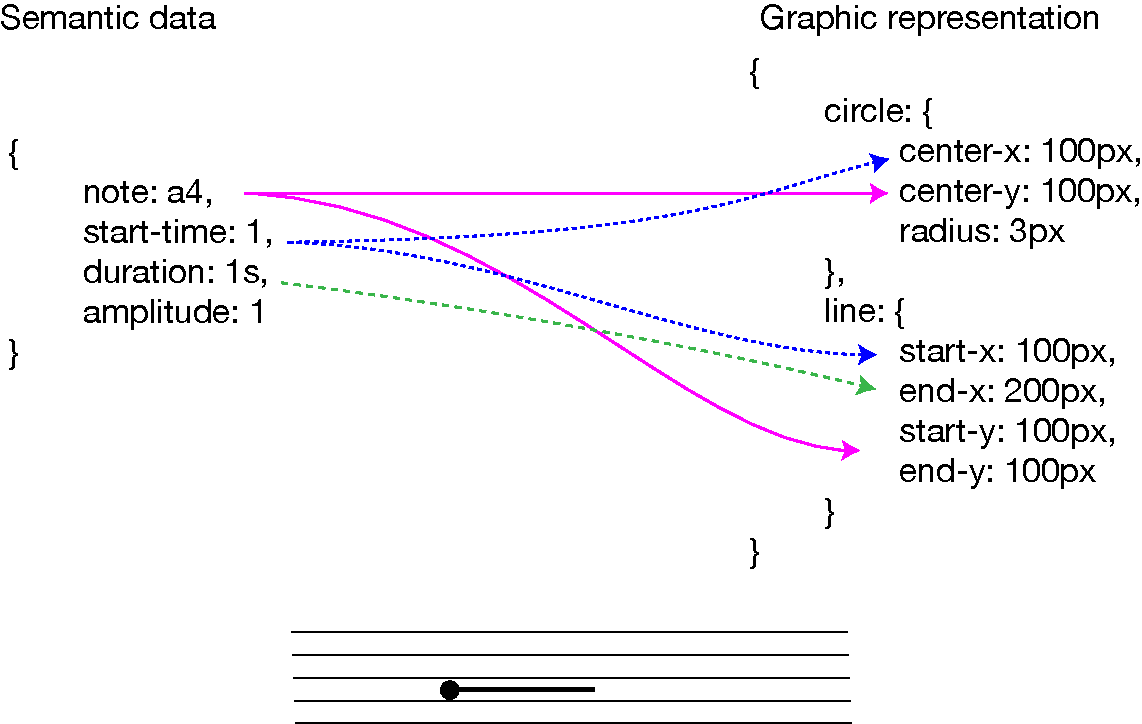
\includegraphics[width=0.9\columnwidth]{data-to-graphic.pdf}
\caption{\textit{semantic data} mapped to create a \textit{graphic} representation from input data.
\label{fig:data-to-graphic}}
\end{figure}

\begin{figure}[ht!]
\centering
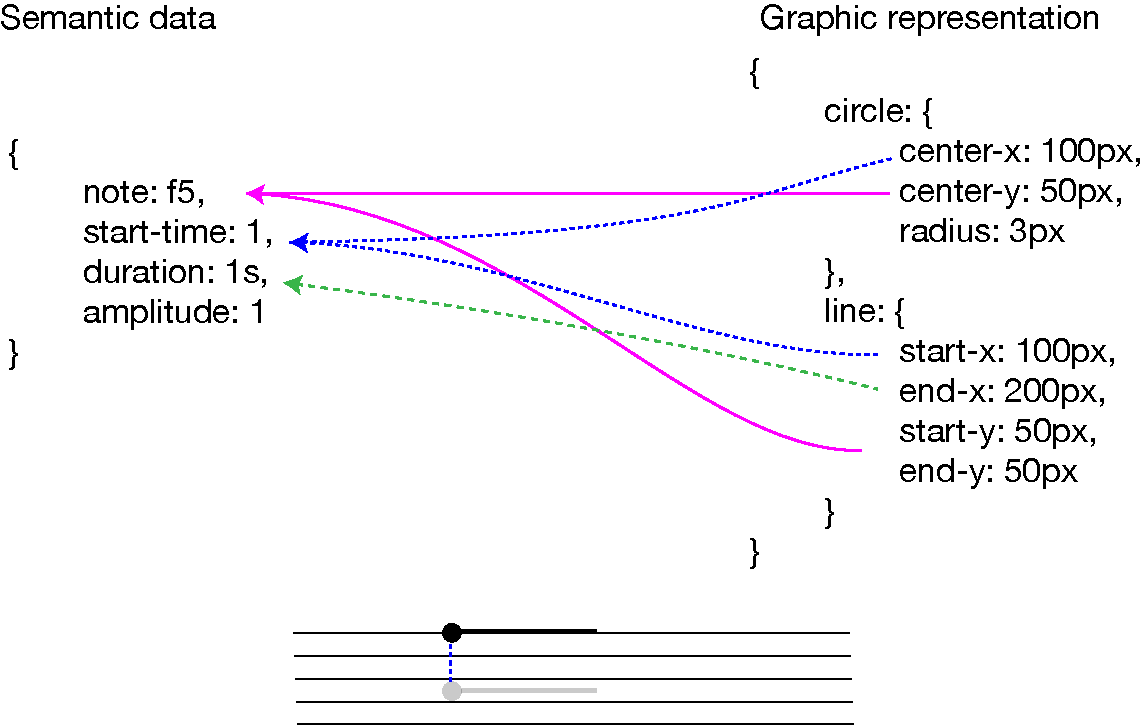
\includegraphics[width=0.9\columnwidth]{graphic-to-data.pdf}
\caption{If edited graphically, the updated graphic data is then mapped back to \textit{semantic data} representation. 
\label{fig:graphic-to-data}}
\end{figure}

\begin{figure}[ht!]
\centering
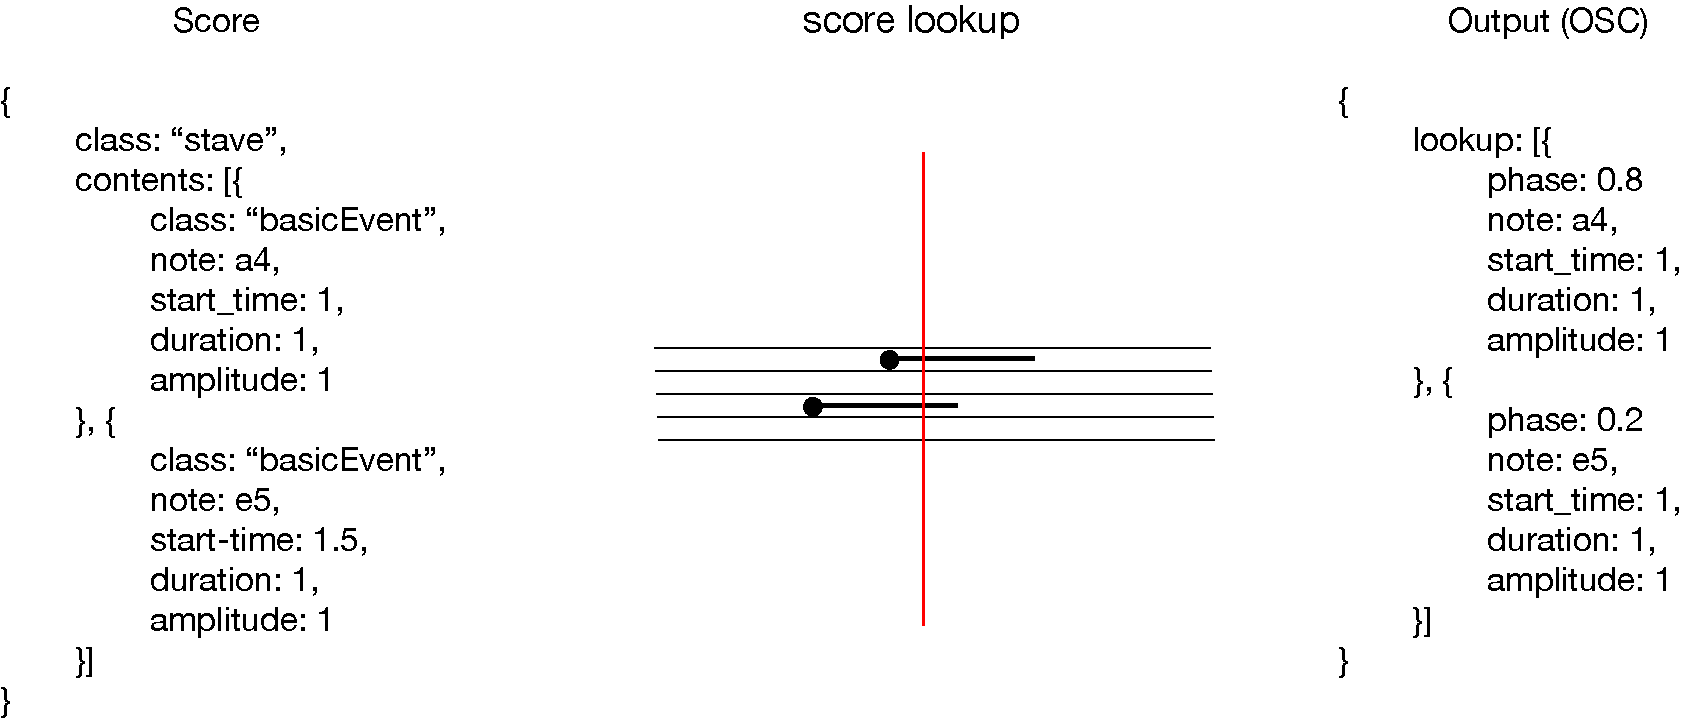
\includegraphics[width=1\columnwidth]{score-lookup.pdf}
\caption{Using the lookup method defined by the symbol class, the \textit{semantic data} can be used to perform external instruments via Open Sound Control. 
\label{fig:score-lookup}}
\end{figure}



\section{Symbol Definitions}\label{library_definitions_api}

Definition scripts are composed as Javascript modules which are loaded into the program at runtime.

Eventually it is planned to provide a set of tools in the GUI for defining a mapping definition graphically but this is not yet implemented.

There are two types of definition scripts:
* `ui` definitions perform user interactions and mapping between semantic data representation and graphic representation.
* `io` definitions are used to assist in the lookup/playback and mapping of the semantic data to media like sound synthesis, video, etc.

Currently, the system uses the same `.js` file to hold both the `ui` and `io` definitions. To aid in development there is a template file that can be used to handle most of the most common actions.


\subsubsection*{io and ui elements}\label{subsec:io_ui_elements}

discuss using DOM elements for hierarchy and js document.querySelector in ui
and similar options in io using score vs model


% internal storage
The data objects is stored in a \textit{model} or \textit{score} which is made up of a hierarchical arrangement of objects called \textit{symbols}.


maybe this should be renamed ..
the main point here is the content aka symbol, which is represented in different ways in different contexts, ui/io aka semantic and graphic versions.

However, since the \textit{ui\_controller} and user definition scripts are all being processed in the browser, scripts are free to use traditional JS approaches to manipulating the browser DOM.

\subsection{Creating Symbols via OSC}

a mechanism for mapping semantic data received from an external application via OSC to symbolic graphic representation; for example by generating scores through algorithmic processes, via textual authoring, via mapping from gestural controller, etc.

using \drawsocket \textit{key/val} message syntax:

\textit{data}: adds a data object to the score, and sends to the ui to be mapped to graphical representation. Parameters include:
\begin{itemize}\itemsep0pt 
  \item \textit{class} (required) the class type of the object to create
  \item \textit{container} (required) the container symbol class to put the object in (in case there are multiple containers that support the same symbol type)
  \item \textit{id} (optional) an id to use for the data object, if non is specified a (long) unique string will be generated.
  \item Other required or optional parameters will depend on the symbol definition.
\end{itemize}

\begin{lstlisting}[ mathescape, columns=fullflexible, basicstyle=\oscfontsize\fontfamily{lmvtt}\selectfont ]
{
    /key : "data",
    /val : {
        /class : "fiveLineStaveEvent",
        /id : "foo"
        /container : "oboe",
        /time : 0.13622,
        /ratio : "7/4",
        /duration : 0.1,
        /amp : 1
    }
  }
\end{lstlisting}



\subsection{API Template SymbolBaseClass }\label{sec:template}


Using the template, a basic definition might look like this:

%
%
%\begin{lstlisting}[
%  mathescape,
%  columns=fullflexible,
%  basicstyle=\oscfontsize\fontfamily{lmvtt}\selectfont,
%]
%const Template = require('../lib/SymbolTemplate') 
%
%class BasicSymbol extends Template.SymbolBase 
%{
%    constructor() {
%        super();
%        this.class = "BasicSymbol";
%    }
%
%
%    get structs () {
%        return {
%
%            data: {
%                class: this.class,
%                id : `\${this.class}-0`,
%                time: 0,
%                pitch: 55,
%                duration: 0.1
%            },
%            
%            view: {
%                class: this.class,
%                id: `\${this.class}-0`, 
%                x: 0,
%                y: 0,
%                r: 2
%            }
%        }
%    }
%
%
%    display(params) {
%
%        ui_api.hasParam(params, Object.keys(this.structs.view) );
%        
%        return {
%            new: "circle",
%            class: 'notehead',
%            id: `\${params.id}-notehead`,
%            cx: params.x,
%            cy: params.y,
%            r: params.r
%        }
%    }
%    
%    getElementViewParams(element) {
%
%        const circle = element.querySelector('.notehead');
%        const x = parseFloat(circle.getAttribute('cx'));
%        const y = parseFloat(circle.getAttribute('cy'));
%        const r = parseFloat(circle.getAttribute('r'));
%
%        return {
%            id: element.id,
%            x,
%            y,
%            r
%        }
%
%    }
%
%
%    getPaletteIcon() {
%        return {
%            key: "svg",
%            val: this.display({
%                id: `circle-palette-icon`,
%                class: this.class,
%                x: 10,
%                y: 10,
%                r: 2
%            })
%        }
%    }
%
%
%}
%
%class BasicSymbol_IO extends Template.IO_SymbolBase
%{
%    constructor()
%    {
%        super();
%        this.class = "BasicSymbol";
%    }
%    
%}
%
%module.exports = {
%    ui_def: BasicSymbol,
%    io_def: BasicSymbol_IO    
%}
%\end{lstlisting}
%


\section{IO Messages}\label{subsec:io_messages}

\symbolist has built in handlers for a set of messages received via OSC, which can be extended by user scripts, using a key/val syntax, where the \textit{key} specifies the function to call, and the \textit{val} are the parameter values to use for the call.

For example, here is a \textit{lookup} query to find elements that are returned by the parameters \textit{time} in the container with the \textit{id} ``trio''.


\begin{lstlisting}[
  mathescape,
  columns=fullflexible,
  basicstyle=\oscfontsize\fontfamily{lmvtt}\selectfont,
]
{
    /key : "lookup:,
    /val : {
        /time : 0.1,
        /id : "trio"
    }
}

\end{lstlisting}

The OSC message API supports the following keys:
\begin{itemize}\itemsep0pt 
\item \textit{data}: adds a data object to the score, and sends to the ui to be mapped to graphical representation. Parameters include:
\begin{itemize}\itemsep0pt 
  \item \textit{class} (required) the class type of the object to create
  \item \textit{container} (required) the container symbol class to put the object in (in case there are multiple containers that support the same symbol type)
  \item \textit{id} (optional) an id to use for the data object, if non is specified a (long) unique string will be generated.
  \item Other required or optional parameters will depend on the symbol definition.
\end{itemize}

\begin{lstlisting}[ mathescape, columns=fullflexible, basicstyle=\oscfontsize\fontfamily{lmvtt}\selectfont ]
{
    /key : "data",
    /val : {
        /class : "fiveLineStaveEvent",
        /id : "foo"
        /container : "oboe",
        /time : 0.13622,
        /ratio : "7/4",
        /duration : 0.1,
        /amp : 1
    }
  }
\end{lstlisting}


\item \textit{lookup}: looks up a point in a container, based on a sorting function specified in the definition. For example, this can be used to get all events active at a given time. Parameters:

\begin{itemize}\itemsep0pt 
  \item \textit{id}: (required) the \textit{id} of the container to lookup in. Containers will generally iterate all child objects, so for example if you use the \textit{id} of the top level score you should be looking up in to all sub-containers.
  \end{itemize}
  
\item \textit{getFormattedLookup}: optional function that might be defined in an \textit{io} script that outputs an object formatted for a different type of player/render. For example, this function might return a list of \textit{/x} and \textit{/y} values for use with the \textit{o.lookup~} Max object, or create a MIDI file export etc. All parameters included in the \textit{val} object will be sent to the \textit{getFormattedLookup} as a parameters object. Parameters:

\begin{itemize}\itemsep0pt 
  \item \textit{id}: (required)
\end{itemize}
\item \textit{call}: calls a function in the one or both of the class definitions. All of the parameters in the \textit{val} object will be passed to the function as an argument. Return values from the \textit{io} controller are with the tag \textit{return/io} and \textit{return/ui} from the \textit{ui}.
\begin{itemize}\itemsep0pt 
  \item \textit{class} (required) class of the object to call
  \item \textit{method} (required) name of object function to call
\end{itemize}

\end{itemize}

\begin{lstlisting}[
  mathescape,
  columns=fullflexible,
  basicstyle=\oscfontsize\fontfamily{lmvtt}\selectfont,
]
{
    /key : "call",
    /val : {
        /function : "functionName",
        /class : "className",
        /id : "foo"
        /someValue : 1,
        /anotherValue : 2
    }
}
\end{lstlisting}

Note that the system will pass the same call to both definitions, so if both have a function of the same name they will both be called.
* \textit{drawsocket}: forwards \drawsocket format messages directly to \drawsocket, bypassing the symbolist mapping.




\section{Case Study}\label{sec:james_score}
hello world!


\section{Conclusions}


\begin{acknowledgments}

\end{acknowledgments} 

%%%%%%%%%%%%%%%%%%%%%%%%%%%%%%%%%%%%%%%%%%%%%%%%%%%%%%%%%%%%%%%%%%%%%%%%%%%%%
%bibliography 
\balance % balance the columns on the last page
\bibliography{symbolist}
\end{document}
